% Co-governed and enforced under the Sovereign Integrity Protocol License (SIP License v1.1):
% https://github.com/tensorrent/ACS-Framework/blob/main/LICENSE
\documentclass[11pt,a4paper]{article}

\usepackage[utf8]{inputenc}
\usepackage[T1]{fontenc}
\usepackage{amsmath,amssymb,amsfonts,amsthm,bm}
\usepackage{booktabs}
\usepackage{microtype}
\usepackage{cite}
\usepackage{xcolor}
\usepackage{float}
\usepackage{tikz}
\usepackage{pgfplots}
\pgfplotsset{compat=1.18}
\usetikzlibrary{arrows.meta, positioning, calc, patterns, decorations.pathreplacing}
\usepackage{geometry}
\geometry{margin=0.60in}
\usepackage{hyperref}

\theoremstyle{remark}
\newtheorem*{remark}{Remark}

\hypersetup{
    colorlinks=true,
    linkcolor=blue!70!black,
    citecolor=green!50!black,
    urlcolor=red!70!black
}

\setlength{\abovedisplayskip}{3pt}
\setlength{\belowdisplayskip}{3pt}
\setlength{\abovedisplayshortskip}{1pt}
\setlength{\belowdisplayshortskip}{1pt}

\newcommand{\dd}{\mathrm{d}}
\newcommand{\ee}{\mathrm{e}}

\title{\LARGE\bfseries Refined $P_\alpha$ Overlap:\\
Parametric Spectroscopic Factor and Self-Consistent WS+Coulomb Eigenmode}

\author{\textbf{ACS Theoretical Physics Working Group}\\[0.3em]
\small\textit{Sovereign-Stack ACS Research Program \& Flag Condensate Project}\\
\small\texttt{research@acs-foundation.org}}

\date{July 23, 2026}

\begin{document}

\maketitle

\begin{abstract}
Two comparison channels extend the throat+Woods--Saxon overlap
proxy~\cite{PalphaThroat2026} on the same 14-isotope set.
\textbf{Channel~A} extracts per-isotope $S_i=P_{\alpha,\mathrm{ext}}/P_{\mathrm{model},i}$
(diagnostic), retains one global $S$, and fits predictive parametric
$\log_{10}S(A,Z)$ and $\log_{10}S(R)$ with leave-one-out (LOO) RMS vs
extracted $\log_{10}P$.
\textbf{Channel~B} replaces the phenomenological WS trial by a
self-consistent $\ell=0$ eigenmode of $V_{\mathrm{WS}}+V_C$ on $[0,R]$
(Dirichlet; depth $V_0$ so $E_0=Q_\alpha$), overlapped with the
throat-weighted flag mode.
On the stated set, parametric $S(A,Z)$ LOO RMS $=0.2862$ reduces
residuals most among \emph{non-tautological} protocols (vs throat+WS
global-$S$ RMS $=0.8247$).  The eigenmode raises Pearson $r$ to
$+0.9676$ but leaves global-$S$ RMS essentially unchanged ($0.8257$).
RC1 scope: documented proxies --- not uniqueness.
\end{abstract}

\vspace{0.1em}
\hrule
\vspace{0.4em}

\section{Motivation}

Reference~\cite{PalphaThroat2026} closed flat$\to$throat/WS geometry and
listed isotope-resolved $S$ and self-consistent WS+Coulomb eigenmodes as
open.  This note implements both as comparison channels on the unchanged
table of~\cite{NuclearDecay2026}.

\begin{remark}[RC1 scope]
Per-isotope $S_i$ zeros that isotope's residual by construction and is
reported only as a diagnostic.  Predictive claims use parametric $S$ with
LOO, or Channel~B with one global $S$.  No uniqueness of many-body
preformation is claimed.
\end{remark}

\section{Radial track layout (DAW metaphor)}
\label{sec:daw-tracks}

Figure~\ref{fig:daw-tracks} is a \emph{schematic} track view of the
refined overlap protocol: horizontal axis $r$ acts as timeline from the
origin through interior support $[0,R]$ to the Coulomb barrier region
$[R,b]$.  Each lane is one radial factor in the throat-weighted overlap
integrand; this is a layout aid only---not a claim that alpha decay is
literally audio production.  In the metaphor, one global spectroscopic
factor $S$ behaves as a master fader on $P_{\mathrm{model}}$; parametric
$S(A,Z)$ is clip-level automation fit per isotope; Dirichlet at $R$
mutes the interior flag lane past the throat wall, whereas Channel~C
routes a Gamow send into $[R,b]$.

\begin{figure}[H]
\centering
\resizebox{\textwidth}{!}{%
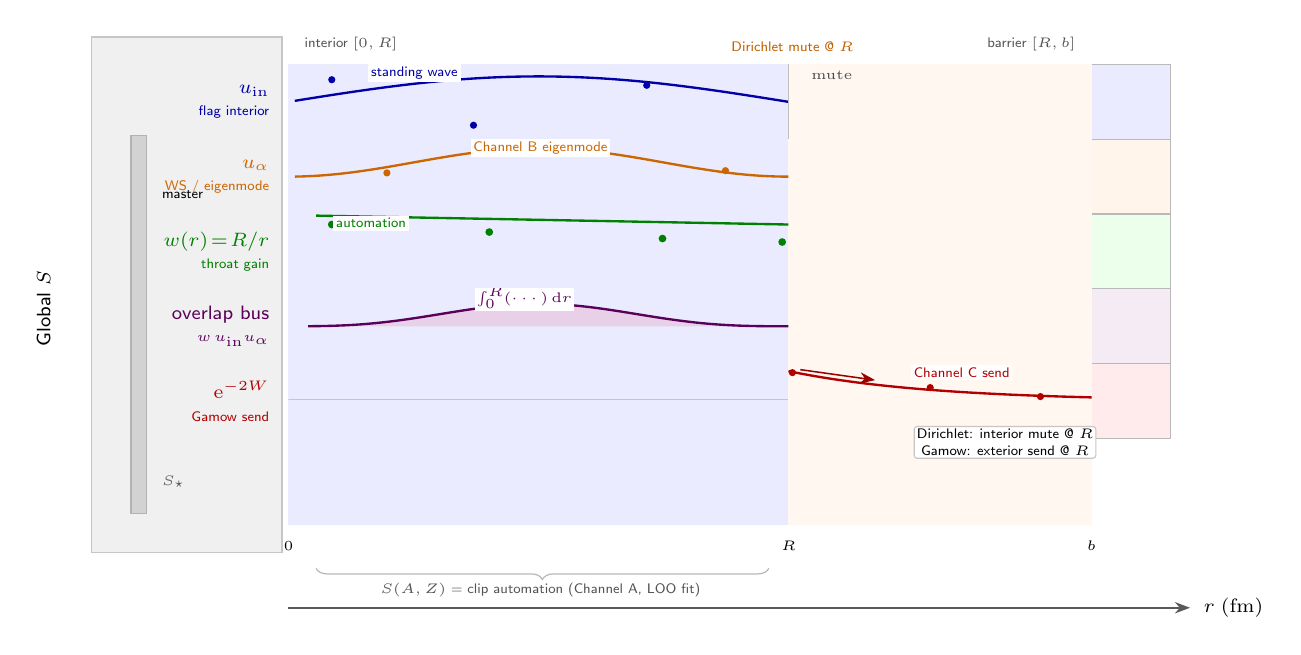
\begin{tikzpicture}[
  track/.style={draw=gray!55, line width=0.4pt},
  hdr/.style={font=\scriptsize\sffamily, anchor=east, align=right},
  tick/.style={font=\tiny, anchor=north},
  ann/.style={font=\tiny\sffamily, fill=white, inner sep=1pt, align=center},
  dot/.style={circle, fill, inner sep=1.2pt},
  >=Stealth
]
  % layout constants
  \def\W{11.2}   % plot width (cm)
  \def\H{0.95}   % lane height (cm)
  \def\HDR{2.35} % header column width (cm)
  \def\xR{6.35}  % throat wall R
  \def\xb{10.2}  % barrier point b
  \def\yTop{5.85}

  % master fader strip (left)
  \draw[fill=gray!12, draw=gray!45, line width=0.5pt]
    (-\HDR-0.15, -0.35) rectangle (-0.08, \yTop+0.35);
  \node[font=\scriptsize\sffamily, rotate=90, anchor=south]
    at (-\HDR-0.55, 2.75) {Global $S$};
  \draw[fill=gray!35, draw=gray!60, line width=0.4pt]
    (-\HDR+0.35, 0.15) rectangle (-\HDR+0.55, 4.95);
  \node[font=\tiny\sffamily, anchor=west] at (-\HDR+0.62, 4.2)
    {master};
  \node[font=\tiny, anchor=west, text=gray!70!black] at (-\HDR+0.62, 0.55)
    {$S_\star$};

  % lane headers + track boxes (top to bottom)
  \foreach \i/\lab/\col/\fillcol in {
    0/{$u_{\mathrm{in}}$\\{\tiny flag interior}}/blue!65!black/blue!8,
    1/{$u_\alpha$\\{\tiny WS / eigenmode}}/orange!80!black/orange!8,
    2/{$w(r)\!=\!R/r$\\{\tiny throat gain}}/green!50!black/green!8,
    3/{overlap bus\\{\tiny $w\,u_{\mathrm{in}}u_\alpha$}}/violet!70!black/violet!8,
    4/{$\ee^{-2W}$\\{\tiny Gamow send}}/red!70!black/red!8
  }{
    \pgfmathsetmacro{\y}{\yTop - \i*\H}
    \draw[track, fill=\fillcol] (0,\y-\H) rectangle (\W,\y);
    \node[hdr, text=\col] at (-0.12,\y-0.5*\H) {\lab};
  }

  % vertical grid + region markers
  \foreach \x/\lab in {0/{0}, 2.2/{}, 4.4/{}, \xR/{$R$}, 7.8/{}, \xb/{$b$}} {
    \draw[gray!25, line width=0.3pt, dashed] (\x,0) -- (\x,\yTop);
    \node[tick] at (\x, -0.08) {\lab};
  }
  \draw[orange!75!black, line width=0.9pt, dashed] (\xR,0) -- (\xR,\yTop);
  \node[ann, text=orange!75!black] at (\xR+0.05, \yTop+0.22)
    {Dirichlet mute @ $R$};
  \fill[blue!8] (0,0) rectangle (\xR,\yTop);
  \fill[orange!6] (\xR,0) rectangle (\xb,\yTop);
  \node[font=\tiny\sffamily, text=gray!65!black, anchor=south west]
    at (0.08, \yTop+0.05) {interior $[0,R]$};
  \node[font=\tiny\sffamily, text=gray!65!black, anchor=south east]
    at (\xb-0.08, \yTop+0.05) {barrier $[R,b]$};

  % --- lane 0: u_in standing wave (mute at R) ---
  \begin{scope}
    \clip (0,\yTop-0*\H-\H) rectangle (\W,\yTop-0*\H);
    \draw[blue!65!black, line width=0.85pt, domain=0.08:\xR, samples=120]
      plot (\x, {\yTop-0*\H-0.5*\H + 0.34*\H*sin(180*\x/\xR)});
    \fill[blue!65!black] (0.55,\yTop-0*\H-0.5*\H+0.34*\H*0.87) circle (1.3pt);
    \fill[blue!65!black] (2.35,\yTop-0*\H-0.5*\H-0.34*\H*0.92) circle (1.3pt);
    \fill[blue!65!black] (4.55,\yTop-0*\H-0.5*\H+0.34*\H*0.65) circle (1.3pt);
    \node[ann, text=blue!65!black] at (1.6, \yTop-0*\H-0.12*\H)
      {standing wave};
    \draw[gray!50, line width=0.5pt] (\xR,\yTop-0*\H-\H) -- (\xR,\yTop-0*\H);
    \node[font=\tiny, text=gray!60!black] at (\xR+0.55, \yTop-0*\H-0.15*\H)
      {mute};
  \end{scope}

  % --- lane 1: u_alpha eigenmode ---
  \begin{scope}
    \clip (0,\yTop-1*\H-\H) rectangle (\W,\yTop-1*\H);
    \draw[orange!80!black, line width=0.85pt, domain=0.08:\xR, samples=100]
      plot (\x, {\yTop-1*\H-0.5*\H + 0.38*\H*sin(180*\x/\xR)*sin(180*\x/\xR)});
    \fill[orange!80!black] (1.25,\yTop-1*\H-0.5*\H+0.05*\H) circle (1.3pt);
    \fill[orange!80!black] (3.55,\yTop-1*\H-0.5*\H+0.32*\H) circle (1.3pt);
    \fill[orange!80!black] (5.55,\yTop-1*\H-0.5*\H+0.08*\H) circle (1.3pt);
    \node[ann, text=orange!80!black] at (3.2, \yTop-1*\H-0.12*\H)
      {Channel~B eigenmode};
  \end{scope}

  % --- lane 2: w(r)=R/r automation gain ---
  \begin{scope}
    \clip (0,\yTop-2*\H-\H) rectangle (\W,\yTop-2*\H);
    \draw[green!50!black, line width=0.85pt, domain=0.35:\xR, samples=80]
      plot (\x, {\yTop-2*\H-0.5*\H + 0.36*\H*(1.35 - 0.35*\x/\xR)});
    \fill[green!50!black] (0.55,\yTop-2*\H-0.5*\H+0.36*\H*1.0) circle (1.4pt);
    \fill[green!50!black] (2.55,\yTop-2*\H-0.5*\H+0.36*\H*0.72) circle (1.4pt);
    \fill[green!50!black] (4.75,\yTop-2*\H-0.5*\H+0.36*\H*0.48) circle (1.4pt);
    \fill[green!50!black] (\xR-0.08,\yTop-2*\H-0.5*\H+0.36*\H*0.35) circle (1.4pt);
    \node[ann, text=green!50!black] at (1.05, \yTop-2*\H-0.12*\H)
      {automation};
  \end{scope}

  % --- lane 3: overlap bus (shaded product) ---
  \begin{scope}
    \clip (0,\yTop-3*\H-\H) rectangle (\W,\yTop-3*\H);
    \fill[violet!18, domain=0.25:\xR, samples=120]
      plot (\x, {\yTop-3*\H-0.5*\H + 0.30*\H*sin(180*\x/\xR)*sin(180*\x/\xR)*sin(180*\x/\xR)})
      -- (\xR,\yTop-3*\H-0.5*\H) -- (0.25,\yTop-3*\H-0.5*\H) -- cycle;
    \draw[violet!70!black, line width=0.85pt, domain=0.25:\xR, samples=120]
      plot (\x, {\yTop-3*\H-0.5*\H + 0.30*\H*sin(180*\x/\xR)*sin(180*\x/\xR)*sin(180*\x/\xR)});
    \node[ann, text=violet!70!black] at (3.0, \yTop-3*\H-0.12*\H)
      {$\int_0^R(\cdots)\,\dd r$};
  \end{scope}

  % --- lane 4: Gamow fade/send past R ---
  \begin{scope}
    \clip (0,\yTop-4*\H-\H) rectangle (\W,\yTop-4*\H);
    \draw[gray!45, line width=0.5pt, domain=0:\xR, samples=2]
      plot (\x, {\yTop-4*\H-0.5*\H+0.02*\H});
    \draw[red!70!black, line width=0.85pt, domain=\xR:\xb, samples=80]
      plot (\x, {\yTop-4*\H-0.5*\H + 0.40*\H*exp(-2.1*(\x-\xR)/(\xb-\xR))});
    \fill[red!70!black] (\xR+0.05,\yTop-4*\H-0.5*\H+0.38*\H) circle (1.3pt);
    \fill[red!70!black] (8.15,\yTop-4*\H-0.5*\H+0.18*\H) circle (1.3pt);
    \fill[red!70!black] (9.55,\yTop-4*\H-0.5*\H+0.06*\H) circle (1.3pt);
    \draw[->, red!60!black, line width=0.55pt]
      (\xR+0.15, \yTop-4*\H-0.5*\H+0.42*\H) -- (\xR+1.1, \yTop-4*\H-0.5*\H+0.28*\H);
    \node[ann, text=red!70!black] at (8.55, \yTop-4*\H-0.12*\H)
      {Channel~C send};
  \end{scope}

  % clip automation callout
  \draw[decorate, decoration={brace, amplitude=4pt, mirror},
        gray!55, line width=0.45pt]
    (0.35, -0.55) -- (\xR-0.25, -0.55);
  \node[font=\tiny\sffamily, text=gray!65!black] at (3.2, -0.82)
    {$S(A,Z)$ = clip automation (Channel~A, LOO fit)};

  % timeline axis
  \draw[->, gray!70!black, line width=0.55pt] (0,-1.05) -- (\W+0.25,-1.05);
  \node[font=\scriptsize\sffamily, anchor=west] at (\W+0.3,-1.05)
    {$r\;(\mathrm{fm})$};

  % send vs mute legend
  \node[ann, draw=gray!45, rounded corners=1pt] at (9.1, 1.05)
    {Dirichlet: interior mute @ $R$\\Gamow: exterior send @ $R$};
\end{tikzpicture}%
}%
\caption{Schematic DAW-style radial track layout for the refined
$P_\alpha$ overlap proxy.  Horizontal axis: radius $r$ from origin
through interior $[0,R]$ to barrier $[R,b]$.  Lanes (top to bottom):
confined flag mode $u_{\mathrm{in}}$ (Dirichlet mute at $R$); alpha
trial or self-consistent eigenmode $u_\alpha$; throat weight
$w(r)=R/r$ as gain automation; overlap bus integrating the weighted
product on $[0,R]$; Gamow envelope $\ee^{-2W(r)}$ as exterior fade/send
(Channel~C).  Global $S$ scales the bus output; parametric $S(A,Z)$
is isotope-resolved clip automation (Channel~A).  Curves are
illustrative, not fitted to a specific isotope.}
\label{fig:daw-tracks}
\end{figure}

\section{Channel A --- isotope $S$ and parametric models}

Base model: throat+WS of~\cite{PalphaThroat2026}
($w=R/r$, Woods--Saxon trial).  Define
\begin{equation}
S_i=\frac{P_{\alpha,\mathrm{ext}}^{(i)}}{P_{\mathrm{model},i}}
=10^{\log_{10}P_{\mathrm{ext}}^{(i)}-\log_{10}P_{\mathrm{model},i}}.
\end{equation}
Global $S_\star=10^{\langle\log_{10}P_{\mathrm{ext}}-\log_{10}P_{\mathrm{model}}\rangle}$
as before.  Parametric fits (least squares):
\begin{align}
\log_{10}S &= b_0 + b_1 A + b_2 Z,\\
\log_{10}S &= c_0 + c_1 R.
\end{align}
Leave-one-out: for each isotope, refit on the other 13 and predict
$\log_{10}S$; LOO RMS is on predicted $\log_{10}(S P_{\mathrm{model}})$ vs
extracted $\log_{10}P$.

\subsection{Channel A numbers (stated set)}
\begin{align*}
\langle S_i\rangle &= 1.001\times 10^{-1}
\quad(\sigma=1.260\times 10^{-1}),\\
\langle\log_{10}S_i\rangle &= -1.4979
\quad(\sigma=0.8558),\\
S_\star &= 3.178\times 10^{-2},\qquad
\mathrm{RMS}_{S_\star}=0.8247,\\
\mathrm{LOO\,RMS}_{S(A,Z)} &= 0.2862,\qquad
\mathrm{LOO\,RMS}_{S(R)}=0.4695.
\end{align*}
Fit (in-sample):
$b_0\approx 14.616$, $b_1\approx +0.0979$, $b_2\approx -0.4312$;
$c_0\approx 48.503$, $c_1\approx -5.435\,\mathrm{fm}^{-1}$.

\section{Channel B --- self-consistent WS+Coulomb eigenmode}

For parent $(A,Z)$ with daughter $(A_d,Z_d)=(A-4,Z-2)$, reduced mass
$\mu$, and nuclear radius $R$ from the table, solve
\begin{equation}
-\frac{\hbar^2}{2\mu}\,u''(r)
+\bigl[V_{\mathrm{WS}}(r;V_0)+V_C(r)\bigr]u(r)=E\,u(r)
\end{equation}
on $[0,R]$ with Dirichlet $u(0)=u(R)=0$ (finite-difference
Sturm--Liouville).  Potentials:
\begin{align}
V_{\mathrm{WS}}&=-\frac{V_0}{1+\ee^{(r-R_{\mathrm{WS}})/a}},
\quad R_{\mathrm{WS}}=r_0 A_d^{1/3},\; a=0.55\,\mathrm{fm},\\
V_C&=
\begin{cases}
\dfrac{Z_\alpha Z_d e^2}{2 R_C}\bigl(3-(r/R_C)^2\bigr), & r<R_C,\\[0.6em]
Z_\alpha Z_d e^2/r, & r\ge R_C,
\end{cases}
\quad R_C=R_{\mathrm{WS}}.
\end{align}
Self-consistency: adjust $V_0$ so the ground eigenvalue $E_0=Q_\alpha$
(box-resonance surrogate; not a complex Gamow eigenphase).  Overlap with
$u_{\mathrm{in}}=r\,j_0(\pi r/R)$ uses throat weight $w=R/r$ as
in~\cite{PalphaThroat2026}.

\subsection{Channel B numbers (stated set)}
\begin{align*}
\langle\log_{10}P_{\mathrm{model}}\rangle &= -0.1110,\\
r\bigl(\log_{10}P_{\mathrm{model}},\log_{10}P_{\mathrm{ext}}\bigr)
&= +0.9676,\\
\mathrm{RMS}_{S=1} &= 2.0237,\qquad
S_\star=1.421\times 10^{-2},\qquad
\mathrm{RMS}_{S_\star}=0.8257.
\end{align*}
Typical fitted depths: $V_0\sim 36$--$43\,\mathrm{MeV}$ on this set
(shallow relative to deep cluster wells --- a consequence of forcing
$E_0=Q_\alpha>0$ under hard-wall Dirichlet at $R$).

\begin{remark}[Boundary condition]
Dirichlet at the throat wall $R$ matches the overlap support of the
confined flag mode.  Channel~C implements outgoing Coulomb/Gamow
matching on $[0,b]$; on the stated 14-isotope set it does not reduce
global-$S$ RMS vs Channel~B (see audit log).
\end{remark}

\section{Acceptance comparison}

\begin{table}[H]
\centering
\caption{Flat / throat+WS / refined eigenmode / parametric $S$ on the
stated 14-isotope set.  LOO applies only to parametric $S$.}
\label{tab:accept}
\scriptsize
\renewcommand{\arraystretch}{0.85}
\begin{tabular}{lcccc}
\toprule
\textbf{Channel} & $\langle\log_{10}P\rangle$ & $r$ & $\mathrm{RMS}_{\mathrm{raw}}$
 & $\mathrm{RMS}_{S_\star}$ / LOO \\
\midrule
flat Gaussian & $-0.3905$ & $+0.8882$ & $1.7705$ & $0.8220$ / --- \\
throat + WS & $-0.4607$ & $+0.8875$ & $1.7099$ & $0.8247$ / --- \\
refined eigenmode & $-0.1110$ & $+0.9676$ & $2.0237$ & $0.8257$ / --- \\
Gamow outgoing & $-0.1110$ & $+0.9676$ & $2.0237$ & $0.8257$ / --- \\
parametric $S(A,Z)$ (LOO) & (base throat+WS) & --- & --- & LOO $0.2862$ \\
parametric $S(R)$ (LOO) & (base throat+WS) & --- & --- & LOO $0.4695$ \\
\bottomrule
\end{tabular}
\end{table}

\begin{remark}[Which channel reduces residuals most?]
Excluding tautological per-isotope $S_i$, \textbf{Channel~A parametric
$S(A,Z)$} yields the largest residual reduction (LOO RMS $0.2862$ vs
global-$S$ RMS $\approx 0.82$).  Channel~B improves correlation
($\Delta r\approx +0.080$) but does not reduce global-$S$ RMS relative
to throat+WS on this set ($\Delta\mathrm{RMS}_{S_\star}\approx +0.001$).
\end{remark}

\section{Artifacts and protocol}

Implementation:
\texttt{rh\_papers\_may21/acs-framework/code/palpha\_overlap/palpha\_overlap\_refined.py}.
JSON:
\texttt{docs/palpha\_overlap\_refined\_results.json}.
Logs:
\texttt{docs/palpha\_overlap\_refined\_logs/}.
Baselines retained:
\texttt{palpha\_overlap.py}, \texttt{palpha\_overlap\_throat.py}.
Gamow channel: \texttt{palpha\_overlap\_gamow.py}.
Extended catalog ($n=29$): \texttt{palpha\_overlap\_extended.py},
\texttt{isotope\_catalog.py}, \texttt{docs/palpha\_overlap\_extended\_results.json}.
Audit: \texttt{docs/palpha\_audit\_log.md}.

\section{Channel C --- Gamow outgoing boundary on \texorpdfstring{$[0,b]$}{[0,b]}}

Channel~B used Dirichlet $u(0)=u(R)=0$ on the throat support.
Channel~C extends the radial domain to $[0,b]$ ($b$ = outer Coulomb
turning point) and replaces the hard wall at $R$ with a Robin outgoing
match at $r=b$ from WKB slope in the exterior allowed region.
Overlap support remains $[0,R]$ with throat weight $w=R/r$.

On the stated 14-isotope set: $r=+0.9676$, $\mathrm{RMS}_{S_\star}=0.8257$
(vs Dirichlet eigenmode $+0.9676$, $0.8257$).  Gamow outgoing BC does
not improve global-$S$ RMS under the documented $E_0=Q_\alpha$ protocol.

\section{Extended isotope catalog (\texorpdfstring{$n=29$}{n=29})}

Fifteen additional alpha emitters from NNDC/NuDat tabulations were added
(see extended JSON metadata).  On $n=29$ throat+WS:
LOO $\mathrm{RMS}_{S(A,Z)}=1.355$ vs $0.286$ on the original 14;
coefficient signs ($b_1>0$, $b_2<0$, $c_1<0$) hold but magnitudes shift.
Parametric $S(A,Z)$ predictive power is scoped to the original stated set
under the mixed extraction protocol in the audit log.

\section{Conclusion}

On the stated set, predictive parametric $S(A,Z)$ with leave-one-out
compresses residual RMS from $\sim 0.82$ (one global $S$) to $0.286$.
A self-consistent WS+Coulomb interior eigenmode improves correlation with
extracted $\log_{10}P$ but does not, by itself, beat throat+WS on
global-$S$ RMS under the documented Dirichlet/$E_0=Q_\alpha$ protocol.
Channel~C (Gamow outgoing on $[0,b]$) likewise leaves global-$S$ RMS
unchanged on the stated set.  Extended catalog ($n=29$) degrades LOO
parametric RMS as documented.  Absolute uniqueness is not claimed.

\begin{thebibliography}{99}
\bibitem{NuclearDecay2026}
  ACS Theoretical Physics Working Group,
  \emph{Nuclear Decay as a Spectral Bifurcation of the Flag Condensate},
  ACS Framework note (2026),
  \texttt{flag\_condensate\_nuclear\_decay.tex}.
\bibitem{PalphaOverlap2026}
  ACS Theoretical Physics Working Group,
  \emph{Standing-Wave Overlap Proxy for Alpha Preformation},
  ACS Framework note (2026),
  \texttt{flag\_condensate\_palpha\_overlap.tex}.
\bibitem{PalphaThroat2026}
  ACS Theoretical Physics Working Group,
  \emph{Throat-Geometry Overlap for Alpha Preformation},
  ACS Framework note (2026),
  \texttt{flag\_condensate\_palpha\_throat\_overlap.tex}.
\end{thebibliography}

\end{document}
